\documentclass[12pt]{amsart}
% packages
\usepackage{graphicx}
\usepackage{setspace}
\usepackage{amssymb,amsmath,amsthm,amsfonts,amscd}
\usepackage{hyperref}
\usepackage{color}
\usepackage{booktabs}
\usepackage{tabularx}
\usepackage{enumitem}
\usepackage[retainorgcmds]{IEEEtrantools}
\usepackage[notref,notcite,final]{showkeys}
\usepackage[final]{pdfpages}
\usepackage{fancyhdr}
\usepackage{upgreek}
\usepackage{multicol}
\usepackage{fontawesome}
\usepackage{halloweenmath}
\usepackage{ytableau}
% set margin as 0.75in
\usepackage[margin=0.75in]{geometry}

% tikz-related settings
\usepackage{tkz-berge}
\usetikzlibrary{calc,quotes}
\usetikzlibrary{arrows.meta}
\usetikzlibrary{positioning, automata}
\usetikzlibrary{decorations.pathreplacing}

%% For table
\usepackage{tikz}
\usetikzlibrary{tikzmark}

% theorem environments with italic font
\newtheorem{thm}{Theorem}[section]
\newtheorem*{thm*}{Theorem}
\newtheorem{lemma}[thm]{Lemma}
\newtheorem{prop}[thm]{Proposition}
\newtheorem{claim}[thm]{Claim}
\newtheorem{corollary}[thm]{Corollary}
\newtheorem{conjecture}[thm]{Conjecture}
\newtheorem{question}[thm]{Question}
\newtheorem{procedure}[thm]{Procedure}
\newtheorem{assumption}[thm]{Assumption}

% theorem environments with roman font (use lower-case version in body
% of text, e.g., \begin{example} rather than \begin{Example})
\newtheorem{Definition}[thm]{Definition}
\newenvironment{definition}
{\begin{Definition}\rm}{\end{Definition}}
\newtheorem{Example}[thm]{Example}
\newenvironment{example}
{\begin{Example}\rm}{\end{Example}}

\theoremstyle{definition}
\newtheorem{remark}[thm]{\textbf{Remark}}

% special sets
\newcommand{\A}{\mathbb{A}}
\newcommand{\C}{\mathbb{C}}
\newcommand{\F}{\mathbb{F}}
\newcommand{\N}{\mathbb{N}}
\newcommand{\Q}{\mathbb{Q}}
\newcommand{\R}{\mathbb{R}}
\newcommand{\Z}{\mathbb{Z}}
\newcommand{\cals}{\mathcal{S}}
\newcommand{\ZZ}{\mathbb{Z}_{\ge 0}}
\newcommand{\cala}{\mathcal{A}}
\newcommand{\calb}{\mathcal{B}}
\newcommand{\cald}{\mathcal{D}}
\newcommand{\calh}{\mathcal{H}}
\newcommand{\call}{\mathcal{L}}
\newcommand{\calr}{\mathcal{R}}
\newcommand{\la}{\mathbf{a}}
\newcommand{\lgl}{\mathfrak{gl}}
\newcommand{\lsl}{\mathfrak{sl}}
\newcommand{\lieg}{\mathfrak{g}}

% math operators
\DeclareMathOperator{\kernel}{\mathrm{ker}}
\DeclareMathOperator{\image}{\mathrm{im}}
\DeclareMathOperator{\rad}{\mathrm{rad}}
\DeclareMathOperator{\id}{\mathrm{id}}
\DeclareMathOperator{\hum}{[\mathrm{Hum}]}
\DeclareMathOperator{\eh}{[\mathrm{EH}]}
\DeclareMathOperator{\lcm}{\mathrm{lcm}}
\DeclareMathOperator{\Aut}{\mathrm{Aut}}
\DeclareMathOperator{\Inn}{\mathrm{Inn}}
\DeclareMathOperator{\Out}{\mathrm{Out}}
\DeclareMathOperator{\Gal}{\mathrm{Gal}}


% frequently used shorthands
\newcommand{\ra}{\rightarrow}
\newcommand{\se}{\subseteq}
\newcommand{\ip}[1]{\langle#1\rangle}
\newcommand{\dual}{^*}
\newcommand{\inverse}{^{-1}}
\newcommand{\norm}[2]{\|#1\|_{#2}}
\newcommand{\abs}[1]{\lvert #1 \rvert}
\newcommand{\Abs}[1]{\bigg| #1 \bigg|}
\newcommand\bm[1]{\begin{bmatrix}#1\end{bmatrix}}
\newcommand{\op}{\text{op}}

% nicer looking empty set
\let\oldemptyset\emptyset
\let\emptyset\varnothing

%the var phi gang
\let\oldphi\phi
\let\phi\varphi

\def\darktheme{} % IAN
\ifx \darktheme\undefined
\else
\pagecolor[rgb]{0.2,0.231,0.302}%{0.23,0.258,0.321}
\color[rgb]{1,1,1}
\fi

\setlist[enumerate,1]{topsep=1em,leftmargin=1.8em, itemsep=0.5em, label=\textup{(}\arabic*\textup{)}}
\setlist[enumerate,2]{topsep=0.5em,leftmargin=3em, itemsep=0.3em}

%pagestyle
%\pagestyle{fancy} 

\begin{document}
\begin{center}
    \textsc{Math 502. HW 3\\ Ian Jorquera}
\end{center}
\vspace{1em}
% See http://www.mathematicalgemstones.com/maria/Math501Fall22.php
% for problems

% sage: https://sagecell.sagemath.org/
\begin{itemize}

\item[(1)] 

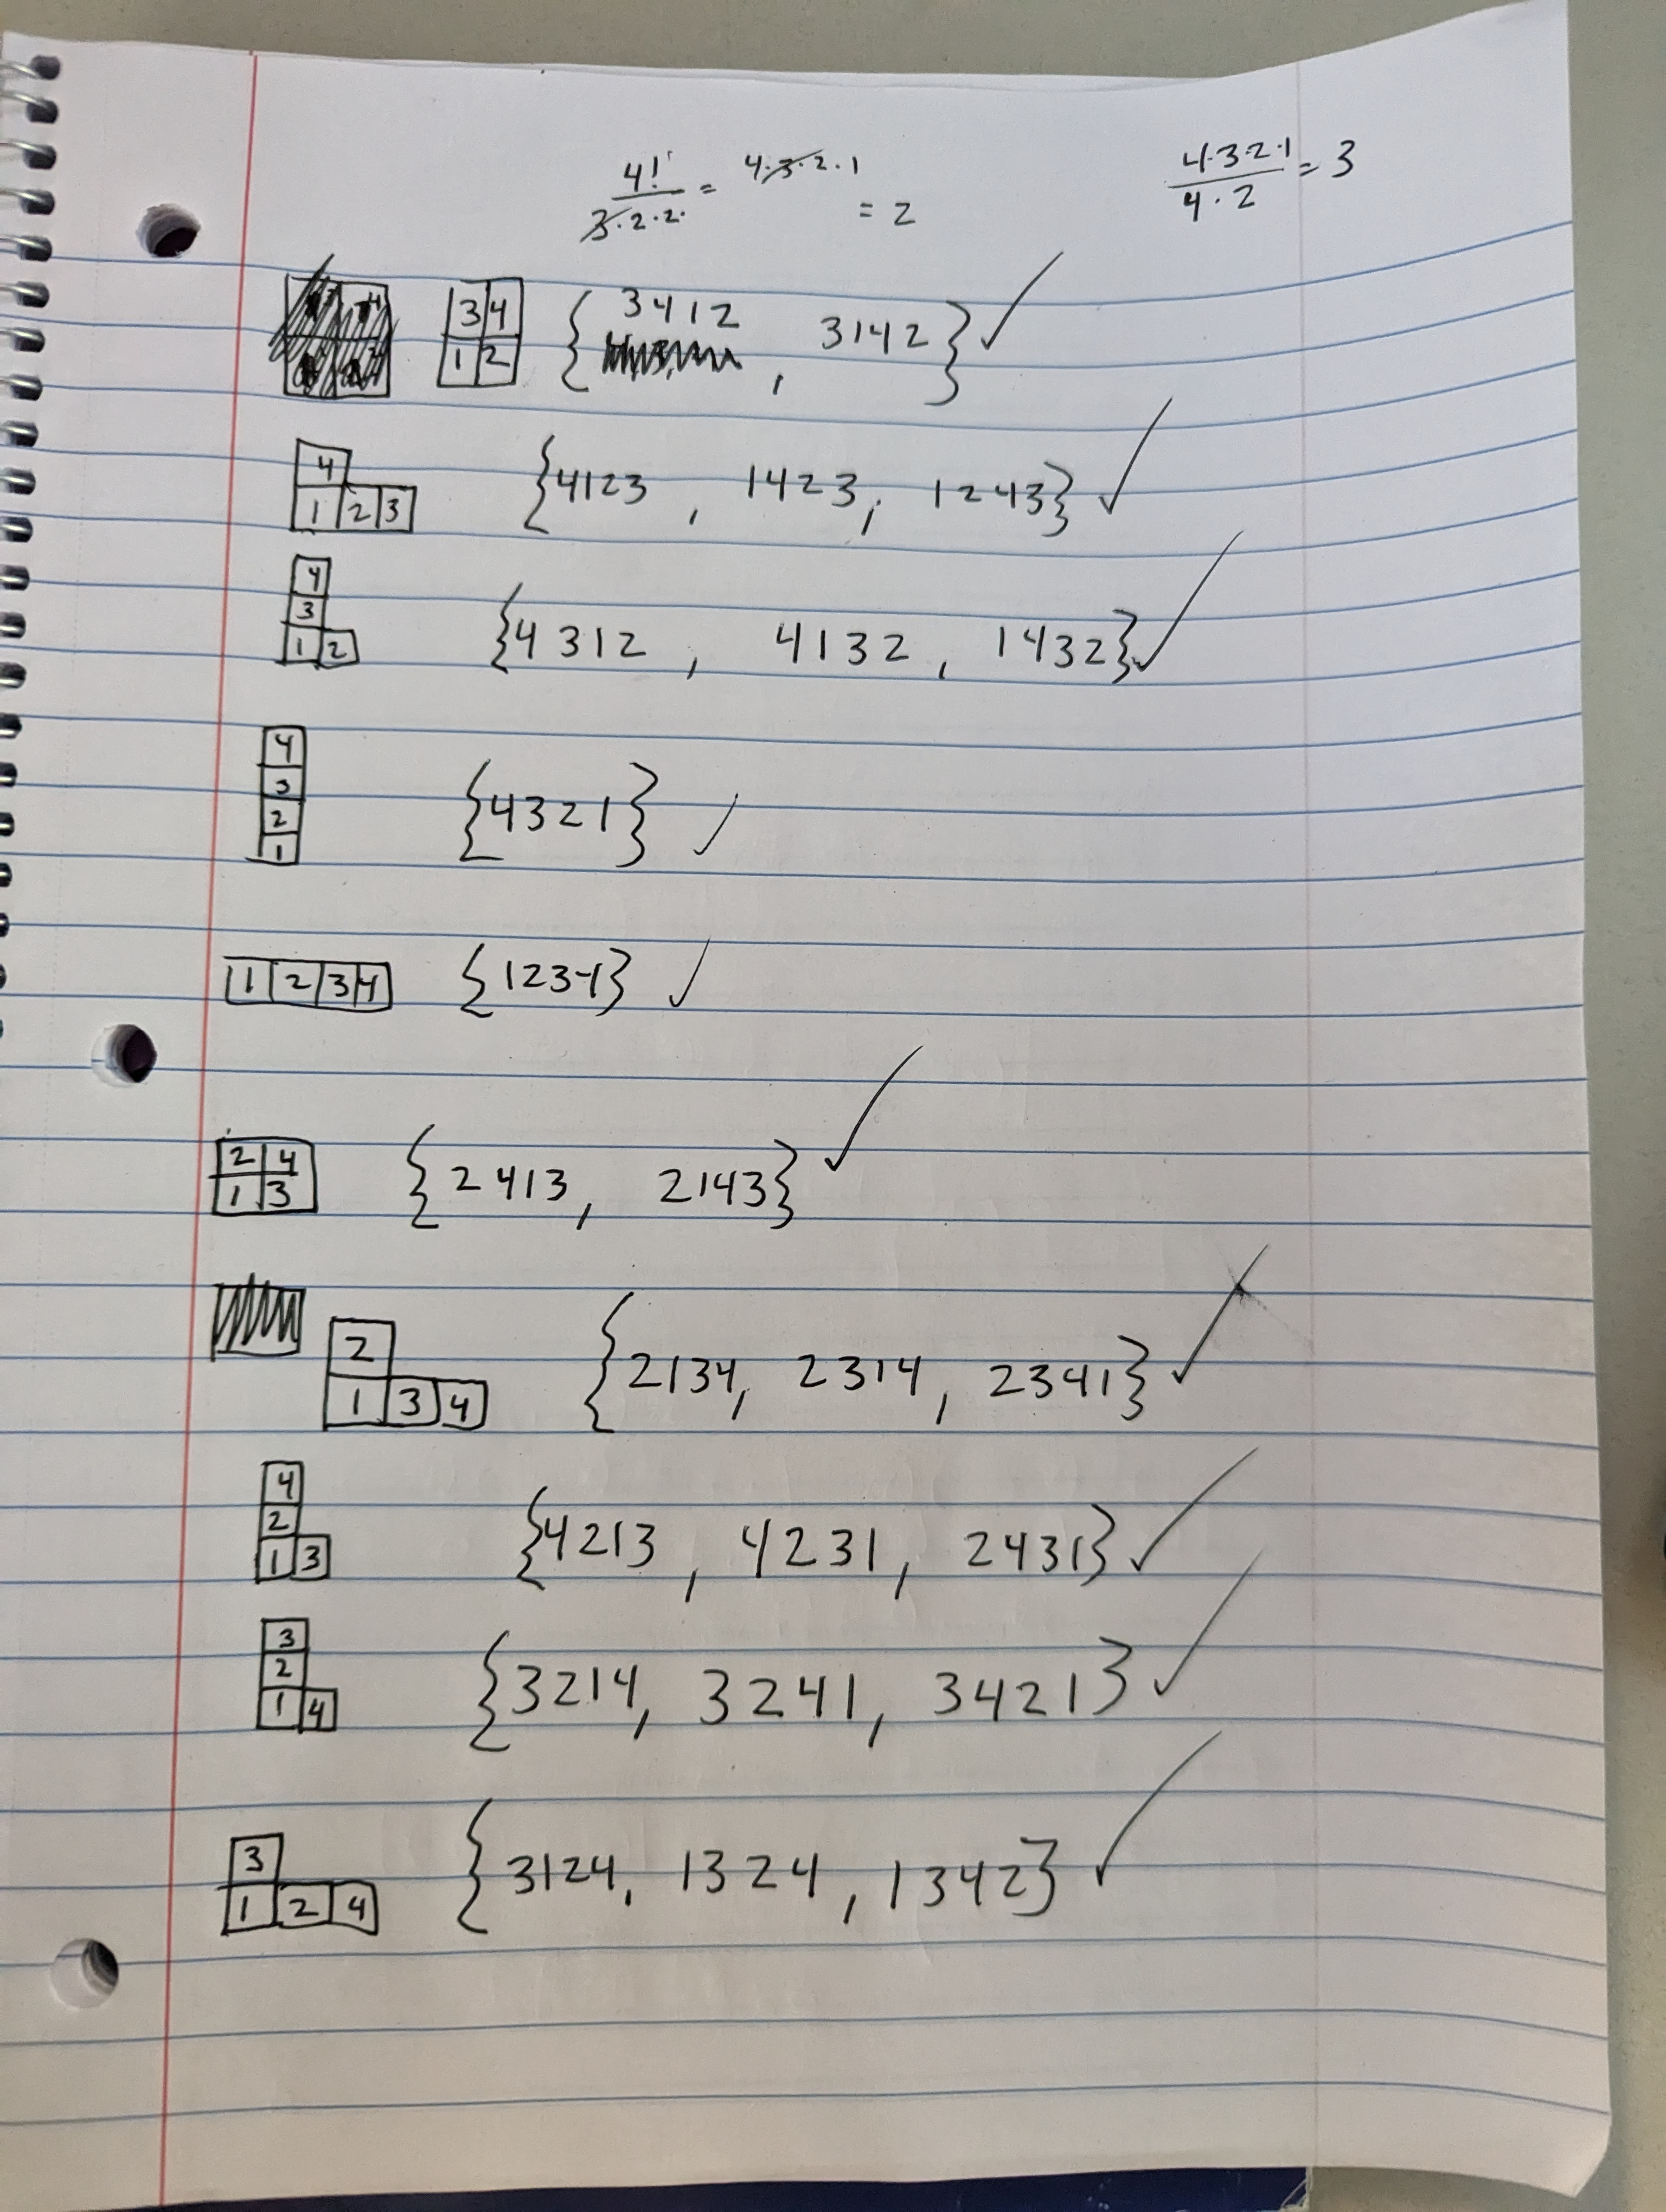
\includegraphics[scale=.1]{pics/hw3PXL_20230208_221932464.jpg}\\

\item[(2)]
\begin{enumerate}[label=(\alph*)]
    \item % [2] (3 points)
    Let $b>a$ and $T$ a semi-standard Young Tableau. We will show that the insertion of $b$ then $a$ into any row of $T$ results $a$ being inserted weakly to the left of $b$ such that $b$ bumps a value $d$ and $a$ bumps a value $c$ such that $d>c$. So consider the insertion of $b$ into a row of $T$. There are two cases. Case 1: $b$ is added to end of the row and bumps no values, meaning $b$ was greater then or equal to all values in the row. In which case $a$ is inserted and bumps the left most value greater then $a$, which in the worst case is the value $b$, as $b$ would work. This means $a$ will be inserted in the same spot or to the left of the previously inserted $b$. Case 2: $b$ is inserted and bumps out a value $d$ that is the left most value strictly greater then $b$, meaning $b$ was greater then or equal to all values in the row to the left of $d$ and strictly less then all values to the right of $d$. In which case $a$ is inserted and bumps the left most value greater then $a$, which in the worst case is the value $b$ as $b$ is greater then $a$. This means $a$ will be inserted in the same spot or to the left of the previously inserted $b$. In this case $a$ would bump a value $c$ which would be a value less then or equal to $b$. Meaning $d>c$.\\

    From the above we can show that the insertions paths of $a$ is weakly to the left of $b$ in $T\leftarrow b\leftarrow a$ where $b>a$. We will show this with induction on the rows, Notice that the insertion $b$ and $a$ into the first row result in $a$ being inserted weakly to the left of $b$ with $a$ bumping $c$ and $b$ bumping $d$ where $d>c$. Then we can repeat this insertion process to the $i$th row where we know that $i-1$th row bumps values $x$ from the $a$ insertion path and $y$ from the $b$ insertions path where $y>x$. And from the above we know that $x$ will be inserted weakly the the left of $y$ and $x$ will bump a value $u$ and $y$ will bump a value $v$ where $v>u$. This means at every row the $a$ insertion path will be weakly to the left of the $b$ insertion path. Notice also that for case 1: where an element of the $b$ insertion path is put at the end of the row and does not bump any elements we have that $a$ will bump a value as it can bump $b$ and its insertion path will continue stricly above the last element in the $b$ insertion path, but no elements above can fall to the right of the last $b$ as the RSK construction creates valid SSYTs. And so the remaining $a$ insertion path will be strictly above and weakly to the left of the last element in the $b$ insertion path.\\

    \item % (1) [1 point]
    Here I have reiterated the last few sentences of the previous part: Notice also that for case 1: where an element of the $b$ insertion path is put at the end of the row and does not bump any elements we have that $a$ will bump a value as it can bump $b$ and its insertion path will continue strictly above the last element in the $b$ insertion path, but no elements above can fall to the right of the last $b$ as the RSK construction creates valid SSYTs. And so the remaining $a$ insertion path will be strictly above and weakly to the left of the last element in the $b$ insertion path.\\

    \item %(1+) [2 points]
    Consider the column tableau with elements $a_m> a_{m-1}>\dots >a_1$ and a SSYT $T$. We will insert the elements $T\leftarrow a_m\leftarrow a_{m-1}\leftarrow \dots \leftarrow a_1$. In order to not have a vertical strip it would have the be the case that two insertions paths end on the same row, as the end of the insertion path is when a new cell in the Tableau is added. However this is not possible as the end of the insertion path for any $a_i$ must be strictly above the end of all previous insertion paths. So no two new cells in the Tableau are added to the same row. And so the result would be a vertical strip.\\
    
    
\end{enumerate}

\item[(4)] %(2) [3 points] 
Let $\pi\in S_n$ and let $\ell$ be the length of the longest increasing subsequence and $d$ the length of the longest decreasing subsequence of $\pi$. Recall that with the RSK algorithm $\pi$ maps to a pair of SYT $(T,S)$ with both the insertion tableau $T$ and the recording tableau $S$ having shape $\lambda$ where $\lambda_1=\ell$ and $\lambda^t_1=d$. This means that the length of bottom row is $\ell$ and the number of rows is $d$. This means that the most cells a valid SYT can have is $\ell d$, and so $n\leq \ell d$ where $n$ is the number of of cells or the size of the permutation.\\

\end{itemize}

\end{document}






